\chapter{Tecniche che fanno uso di altri segnali}
In questa parte verranno descritte delle tecniche che sono state progettate per usare altri seganli al di furi del contenuto delle pagine web e della struttura del grafo. La continua evoluzione delle tecniche di spam web ha portato una consecutiva crescita è innovazione nell'ambito dello sviluppo di tecniche di spam detection. Molte delle tecniche sviluppate per cercare di identificare tutti i vari tipi di spam sono state progettate con l'intento di essere un supporto alle tecniche già presenti in letteratura. Molte tecniche basate sul contenuto fanno uso di feature che si basano su euristiche che sono state calcolate su alcuni dataset a disposizione mentre le tecniche che fanno uso del grafo cercano di diminuire o eliminare del tutto l'effetto dei nodi spam identificando dei specifici pattern. Per cercare di indetificare i tipi di pagine web spam che non si riesce ad identificare con i precedenti metodi sono state sviluppate nuove tecniche.

\section{Link dai forum}
Gli spammer utilizzano i forum SEO (Search Engine Optimization) per creare link spam, infatti utilizzano questi strumenti web per la condivisione e lo scambio di link. Alcuni metodi di spam detection vanno a cercare i link che vengono scambiati tra gli spammer propio in questi forum \cite{Cheng:2011:LWS:1935826.1935902} e utilizzano questi link per rilevare lo spam; in effetti tale metodo fa parte delle tecniche che utilizzano segnali come il grafo del web ma dato che il modo in cui vengono rilevati i siti spam è inusuale allora venie catalogato tra i metodi che fanno uso di altri segnali. Tale processo non è semplice in quanto nei post dei forum ci sono altre informazioni che producono rumore nel rilevamento dei link. Per rendere efficiente il metodo si eseguono le seguenti operazioni:
\begin{itemize}
 \item vengono estratti tutti i link contenuti nei post.
 \item vengono estratte le feature dai link sulla base delle loro relazioni con gli utenti del forum e della struttura dei loro link nel grafo del web. Le feature vengono catalogate in tre tipi: feature del forum SEO (quali la frequenza di URL nel forum, numero di thread che il proprietario dell'URL ha discusso, numero di post autorizzati dal proprietario dell'URL, numero di URL inseriti dal proprietario dell'URL, media degli URL per post di un utente, numero di post che contengono l'URL del proprietario), feature del grafo (fanno parte il numero di link in ingresso, numero di link in uscita, media dei link in uscita dei vicini in ingresso, media dei link in entrata dei vicini in uscita) e feature del sito (la lunghezza dell'URL). 
 \item viene utilizzato un framework per calcolare il valore di spam dei siti.
\end{itemize}
Questi metodi sono di particolare aiuto nell'incrementare il numero di pagine spam che i metodi convenzionali (sia basati sul contenuto che sulla struttura del grafo) non riescono a identificare  e perciò è possibile usarlo come metodo complementare ai metodi classici.

\section{Rilevamento dello spam di tipo cloacking}
Ci sono pochi metodi che tentano di rilevare il cloaking. Gli spammer possono rilevare un crawler dal suo indirizzo IP o dal campo \textit{user-agent} all'interno di una richiesta HTTP e quindi fornire due versioni di una pagina a seconda di chi effettua la richiesta.Alcuni metodi per rilevare il cloaking prendono in considerazioni due copie di una stessa pagina, la prima  quella ottenuta tramite un crawler mentre la seconda è quella ottenuta da un browser. Le due copie successivamente vengono confrontate per verificare se le due pagine siano identiche le stesse e quindi che non si tratti di cloacking. I metodi che fanno uso di questa tecnica non sono efficaci per il fatto che oggi le pagine vegono generate dinamicamente e possono variare nei contenuti. Un metodo, che riesce a superare questa problematica, si basa sul confronto dei termini tra le due copie di una pagina usando delle funzioni hash per aumentare la velocità di confronto \cite{Ghiam:2013cloaking}. Sia \(C_i\) le copie di una pagina che sono 
ritornate ad un crawler e \(B_i\) le copie di una pagina che sono ritornate ad un browser e sia \(f\) una funzione hash come MD5 allora \(f(B_i)\) e \(f(C_i)\) sono i valori di hash rispettivamente delle copie del browser e del crawler; se i valori delle funzioni hash sono identici allora le pagine sono identiche. L'algoritmo contradistingue il cloacking in statico e dinamico. Nel primo caso ci si trova nella situazione in cui le copie di una pagina del browser e del crawler sono diverse, per determinare tale tipo di cloaking l'algoritmo segue 5 passaggi:
\begin{itemize}
 \item La prima fase valuta \(f(C_1)\) e \(f(B_1)\) se i due valori di hash sono differenti vengono calcolati anche \(f(B_2)\) e \(f(C_2)\). Valori di hash differenti implicano una buona probabilità che le due pagine derivino da un meccanismo di cloacking, ma queste considerazioni non sono sufficienti perciò bisogna eseguire il passo successivo.
 
 \item In questa fase i valori di hash vengono valutati nel seguente modo: \(f(C_1)\not =f(B_1)\), \(f(C_2)\not=f(B_2)\), \(f(C_1)=f(C_2)\), \(f(B_1)=f(B_2)\). Tale valutazione suggerisce che la probabilità di cloacking è elevata ma data l'alta natura dinamica delle pagine web per essere sicuri di essere di fronte ad un meccanismo di cloacking si calcola la differenza dei termini tra \(C_1\) e \(B_1\) (denominata \(D_{C1B1}\)) che se è minore di una certa soglia allora indica che non si tratta di cloacking.
 
 \item La terza fase si contradistingue dal caso in cui \(f(C_1)\not=f(B_1)\), \(f(C_2)\not=f(B_2)\), \(f(C_1)=f(C_2)\), \(f(B_1)\not=f(B_2)\). Questo caso si differenzia dal precedente per il fato che le due copie del browser sono diverse questo suggerisce che la probabilità di cloacking è bassa e che si tratti di un contentuto altamente dinamico. Per prevenire falsi positivi vengono viene calolata \(D_1\) come le differenze dei termini tra \(C_1\) e \(B_1\) e \(D_2\) come le differenze dei termini tra \(C_2\) e \(B_2\) e succesivamente \(D_{TOTAL}\) come la differenza tra \(D_1\cup D_2\) e \(D_1 \cap D_2\). Se \(D_{TOTAL}\) è più grande di una certa soglia allora ci si trova davanti un meccanismo di cloacking.
 
 \item La quarta fase si ha con \(f(C_1)\not=f(B_1)\), \(f(C_2)\not=f(B_2)\), \(f(C_1)\not=f(C_2)\), \(f(B_1)\not=f(B_2)\), dal momento che \(f(C_1),f(C_2),f(B_1),f(B_2)\) sono differenti queste pagine cambiano molto velocemente sono pagine dinamiche. 
 
 \item Infine \(f(C_1)\not=f(B_1)\), \(f(C_2)\not=f(B_2)\), \(f(C_1)\not=f(C_2)\), \(f(B_1)=f(B_2)\), in questo caso esiste una buona probabilità di cloacking. Per determinare se la differenza tra le due copie del crawler e l'identicità tra le copie del browser indicano che si tratta di cloacking viene calcolato \(D_{C1C2}\) come la differenza dei termini tra le copie del crawler e \(D_{B1C1}\) come la differenza dei termini tra \(B_1\) e \(C1\). Se \(D_{C1C2}\) e maggiore di \(D_{B1C1}\) allora non si tratta di cloacking perchè la differenza tra le copie del crawler e maggiore della differenza tra la copia del crawler e quella del browser; questo sta a sottolineare la natura dinamica della pagina.
\end{itemize}
Per determinare il cloacking dinamico ovvero quando si incombe in questa situazione \(B_1=B_2=C_2 \not =C_1\) vengono definite 2 fasi:
\begin{itemize}
 \item Il caso in cui \(f(C_1)\not=f(B_1)\), \(f(C_2)=f(B_2)\), \(f(B_1)\not=f(B_2)\). In questo caso non si può parlare di cloacking in quanto \(f(B_1)\) è diverso di \(f(B_2)\) ovvero già le due copie del browser sono diverse e quindi si tratta della pagina che cambia i contenuti ma non per fare cloacking.
 \item Nel secondo caso \(f(C_1)\not=f(B_1)\), \(f(C_2)=f(B_2)\), \(f(B_1)=f(B_2)\) ovvero nella situazione del cloacking dinamico si nota che nel primo caso le copia \(C_1\) del crawler e quella \(B_1\) del browser sono diverse mentre nel secondo caso la copia del crowler \(C_2\) è uguale alla copia del browser \(B_2\). Questo significa o che il server spam sceglie quando effettuare il cloacking o che c'è una relazione con la natura dinamica delle pagine. Per questo l'algoritmo prevede il calcolo di \(D_{C1C2}\) che è uguale alla differenza dei termini tra le due copie del crawler. Se \(D_{C1C2}\) è maggiore di una certa soglia allora si tratta di cloacking.
\end{itemize}

\section{Rilevare lo spam tramite l'header HTTP}
Un metodo innovativo per rilevare lo spam è quello descritto in \cite{Webb:2008:PWS:1458082.1458129}. Tale metodo può essere usato come supporto ad altri metodi descritti in precedenza e può essere utilizzato in modo dinamico duranti la fase di scaricamento delle pagine, utile per risparmiare il numero di richieste inutili verso pagine spam. Diversamente dai metodi classici (basati sull'uso del contenuto della pagina o sulla struttura del grafo) questo metodo utilizza le informazioni racchiuse all'interno dell'header HTTP per determinare le pagine spam. Oltre all'utilizzo lato server (crawler) può essere usato anche lato client per migliorare la qualità dei contenuti protegendo da malware e permettendo di riparmiare banda e quantità di memoria. Infatti prima viene effetuata una richiesta HTTP, al server, per una pagina ma durante la lettura della pagina ci si ferma al solo header; successivamente viene azionato un classificatore per valuare l'header come spam o non spam; se l'header viene classificato come 
non spam allora si continua con la lettura del resto della pagina. I vari campi all'interno delle sessioni HTTP possono essere usate come feature che sono poi valutate dal classificatore. Analizzando i vari campi si nota che le pagine spam hanno molto frequentemente alcuni campi rispetto alle pagine non spam che hanno gli stessi campi con minore probabilità. Ad esempio in figura \ref{img:webb1} vengono confrontate le distribuzioni degli indirizzi IP per il corpus di pagine WebSpam (che contiene delle pagine spam) e il corpus WebBase (che contiene pagine non spam); dal grafico si nota che gli indirizzi IP nel corpus WebSpam sono concentrati principalmente nel range tra \(63.* - 69.*\) e \(204.* - 216.*\).
\begin{figure}
\centering
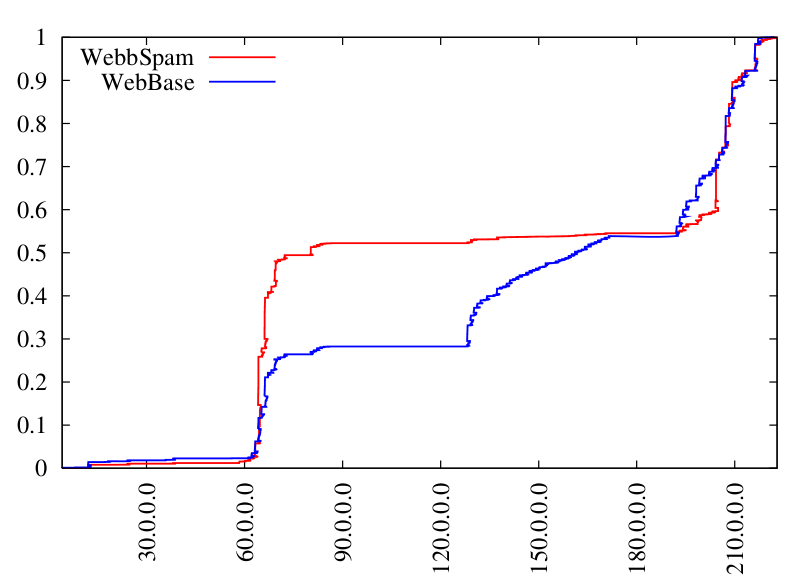
\includegraphics[width=10cm]{immagini/altre/webb.png}
\caption{Distribuzione degli indirizzi IP di due dataset: WebSpam che contiene pagine spam e WebBase che contiene pagine non spam.}
\label{img:webb1}
\end{figure}
Perciò tale metodo tenta di fare uso dell'header HTTP in modo tale da classificare le pagine basandosi sull'osservazione che pagine spam e pagine non spam	 hanno valori (campi dell'header) che hanno distribuzioni distinte. Questo metodo comunque non è molto affidabile se usato da solo perciò è un ottimo strumento da usare in modo complementare ad altri metodi più tradizionali. Un uso sensato sarebbe quello di utilizzare questa tecnica come processo di preselezione in modo tale da sfoltire il numero di pagine che gli altri metodi (che si basano o sull'uso del contenuto delle pagine o del grafo del web) devono utilizzare e quindi richiedendo un numero minore di risorse.

\section{Altri metodi}
Oltre ai metodi descritti fino adesso esistono altri che fanno uso di diversi tipi di segnali per identifcare lo spam. La motivazione nasce dal fatto che le tecniche di spaming cambiano continuamente in modo tale da ingannare i motori di ricerca. I metodi che non fanno uso del contenuto della pagina web o del grafo del web nascono appunto con l'intento di rilevare le nuove forme di spam o lo spam che i metodi classici non riescono a rilevare. Ad esempio alcuni metodi fanno uso di pattern basati sul comportamento dell'utente per identificare le pagine spam. In \cite{Liu:2008:UBO:1367497.1367645}  è descitto un metodo che identifica le pagine spam che fa uso di tre feature ricavate da pattern comportamentali basati sulle azioni dell'utente in presenza di  pagine spam e pagine non spam. Le feature sono cosi calcolate:
\begin{itemize}
 \item La prima feature è denominata SEOV (Search Engine Oriented Visit) ed è definita come:
 \begin{equation}
  SEOV(p)=\frac{\#(Search\ engine\ oriented\ visit\ of\ p)}{\#(Visit\ of\ p)}
 \end{equation}
  dove \(p\) rappresenta la pagina web per cui viene calcolata la feature. La misura al numeratore indica la visita della pagina \(p\) per mezzo dei motori di ricerca mentre la misura denominatore indica la visita alla pagina \(p\) senza il bisogno di utilizzare i motori di ricerca. Dato che un utente non andrebbe mai su pagine spam se non ingannato dai risultati dei motori di ricerca, le pagine spam hanno valori alti per questa feature. In figura \ref{img:seov} è rappresenta la distribuzione delle pagine (del dataset usato dagli autori) sulla base del valore della feature SEOV; in rosso sono rappresentate le pagine spam mentre in blu sono rappresentate le pagine non spam. Molte pagine web spam hanno valori SEOV più alti delle pagine non spam perchè i motori di ricerca sono gli strumenti, e in alcuni casi sono gli unici, tramite cui le pagine spam possono essere raggiunte.
\begin{figure}
\centering
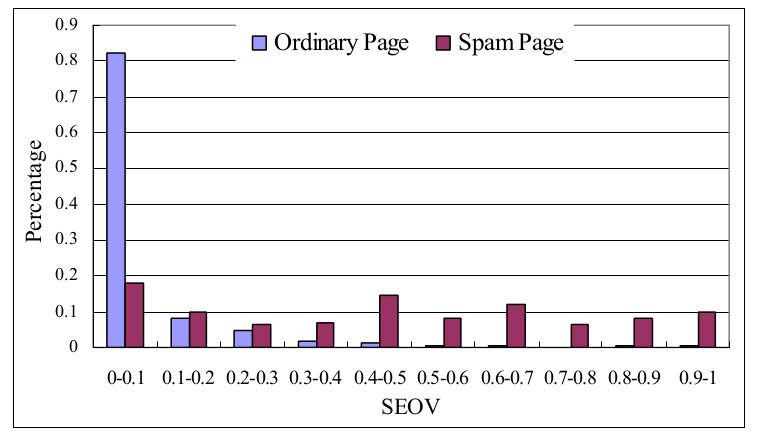
\includegraphics[width=10cm]{immagini/altre/seov.png}
\caption{Distribuizione delle pagine sulla base della feature SEOV.}
\label{img:seov}
\end{figure}
  
 \item Visto che esiste una grande differenza tra chi progetta una pagina spam e chi ne progetta una non spam, ci si avvale del comportamento dell'utente per etichettare le pagine. Un utente rimane su una pagina spam solo fino a al punto in cui capisce di essere su un sito con contenuti non pertinenti, mentre nel caso in cui si trovi a navigare su una pagina non spam l'utente è stimolato a rimanrci. Quindi la seconda feature è definita come SP (Start Point Visiting rate):
 \begin{equation}
  SP(p)=\frac{\#(user\ click\ a\ hyperlink\ on\ p\ while\ visiting\ p)}{\#(Visit\ of\ p)}
 \end{equation}
 questa feature indica quanti click sono fatti su una certa pagina \(p\).
 \item Infine l'ultima feature è denominata SN (Short-term Navigation rate) e indica quante pagine di un sito \(w\) saranno visitate una volta che un utente visita il sito \(w\). Questa misura è definita in questo modo:
 \begin{equation}
  SN(w)=\frac{\#(Session\ in\ wich\ users\ visit\ less\ than\ N\ pages\ in\ w)}{\#(Session\ in\ wich\ user\ visit\ w)}
 \end{equation}
 \end{itemize}
Qundi questo metodo utilizzando pattern comportamentali per determinare le pagine spam è molto più flessibile dei metodi tradizionali, i quali sono dipendenti dalla struttura della pagina o del grafo. La novità di questo metodo sta nel fatto che mentre gli altri metodi sono basati sullo studio di determinate proprietà che le pagine web hanno (nel caso dei metodi basati sul contenuto delle pagine) o sullo studio del grafo del web e la tipologia che le pagine web assumo all'interno quest'ultimo metodo si basa sul comportamento dell'utente. Questo rende il problema dell'identificazione dello spam scalabile ovvero protrebbe riuscire ad arginare e rilevare anche le nuove tipologie di spam web che potrebbero essere implementate mentre con i metodi classici è più difficile in quanto si basano su delle euristiche riscontrate su alcuni dataset e quindi sono dipendenti dalla tipologia di spam che si riscontra e non sono mutabili ovvero non possono essere flessibili per apprendere i nuovi tipi di tecniche spam.

Ci sono altri metodi che fanno uso del comportamento dell'utente durante la navigazione web per determinare le pagine spam molto innovativo e interessante è \textit{BrowseRank} \cite{Liu:2008:BLW:1390334.1390412}. \textit{BrowseRank} determina l'importanza di una pagina web dal grafo ricavato dal comportamento dell'utente durante la navigazione web con il browser. Il grafo è costituito dai vertici che rappresentano le pagine. da archi orientati che rappresentano le transizioni da una pagina all'altra da parte dell'utente e anche dal tempo di permanenza su una pagina. Infine come per \textit{Pagerank} viene utilizzato il grafo ricavato per determinare l'importanza delle pagine. In figura \ref{img:browser} è rappresentato uno schema esplicativo del modo con cui si ricava il grafo. Il grafo è ricavato dai browser degli utenti (ad esempio tramite l'utlizzo di toolbar) che raccolgono diversi dati come l'URL, il tempo di permanenza, la tipologia della visita (ad esempio se l'utente ha inserito l'URL nella barra degli indirizzi del browser oppure se arrivato a ad una pagina per mezzo di un link) e vegono poi recuperati da un server che integra i dati provenienti da milioni di utenti.
\begin{figure}
\centering
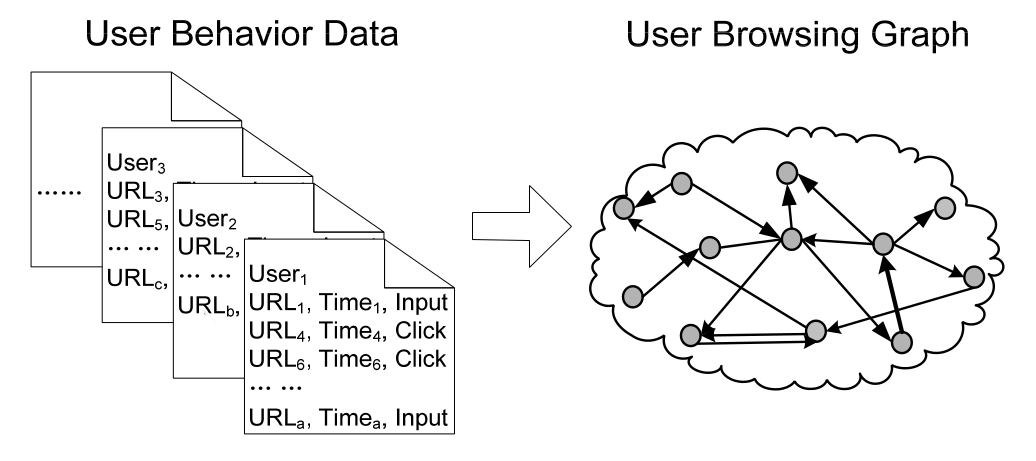
\includegraphics[width=10cm]{immagini/altre/browser.png}
\caption{Dal comportamento dell'utente al grafo.}
\label{img:browser}
\end{figure}
Questo algoritmo ha due vantaggi principali rispetto ai metodi tradizionali sui link quali:
\begin{itemize}
 \item Dato che il grafo è ricavato durante la fase di navigazione è più accurato di quello ricavato da un crawler perché i link tra le pagine possono cambiare continuamente.
 \item Questo metodo inoltre tiene conto anche del tempo in cui ci si sofferma su una pagina, caratteristica che può fare capire se si è in presenza di una pagina spam, infatti un utente non avrebbe nessun vantaggio a rimanere a lungo su una pagina con poca pertinezza e qualità rispetto al suo bisogna di informazione.
\end{itemize}
Dagli esperimenti gli autori hanno notato che \textit{BrowseRank} è più efficiente rispetto a \textit{Trustrank} e quindi dimostra che i metodi che si basano su segnali differenti dal contenuto o dal grafo del web possono essere in grado di lavorare autonomamente e non solo in modo  complementare ai metodi classici.

Un ultimo metodo \cite{Wei:2012:FAW:2348283.2348338} per rilevare lo spam web affronta  il problema da un altro punto di vista: gli autori hanno osservato che le query più comuni (quelle che hanno un alta frequenza nei file log dei motori di ricerca) sono  quelle che genereranno più spam. Tali query hanno le seguenti caratteristiche: sono molto comuni e quindi riflettono una grande quantità di richiesta da parte degli utenti, e i risultati per queste query sono composti da pochi risultati utili in quanto sono prese di mira per fare spam ovvero le pagine spam molte volte sono piene di pubblicità e per attirare l'utente (o meglio per ingannarlo) cercano di manipolare i motori di ricerca per andare in cima ai risultati quindi le query più popolari saranno prese di mira più frequentemnte da chi fa spam. Il metodo, tenendo conto di queste considerazioni, fa uso dei file log dei click dei motori di ricerca per prevenire lo spam web.
